%!TEX root = ../2018_06_13-HATS-LPC-JEC.tex

\subsection{Textfile Format}

\frame{
\frametitle{What form do the corrections come in?}
\framesubtitle{JEC Text Files}
                \begin{figure}
                  \centering
		     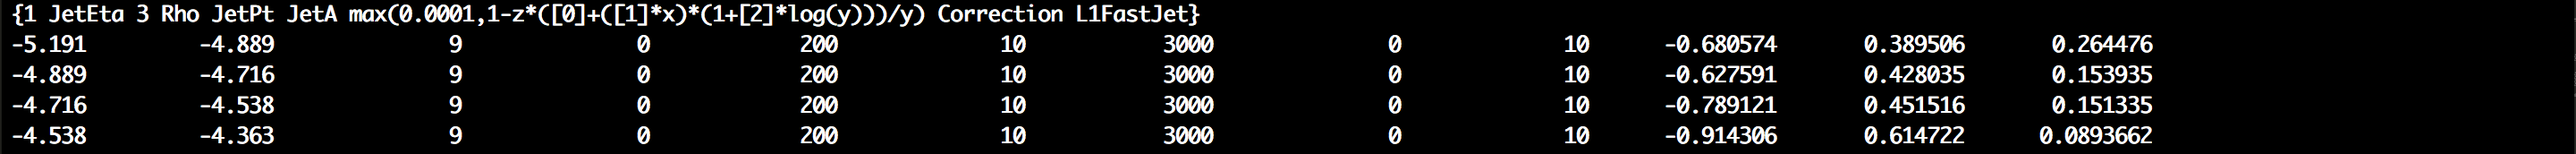
\includegraphics[width=\textwidth]{images/TextFileScreenshots/L1FastJet.png}    
                    \caption{L1FastJet}
                 \end{figure}

                \begin{figure}
                  \centering
		     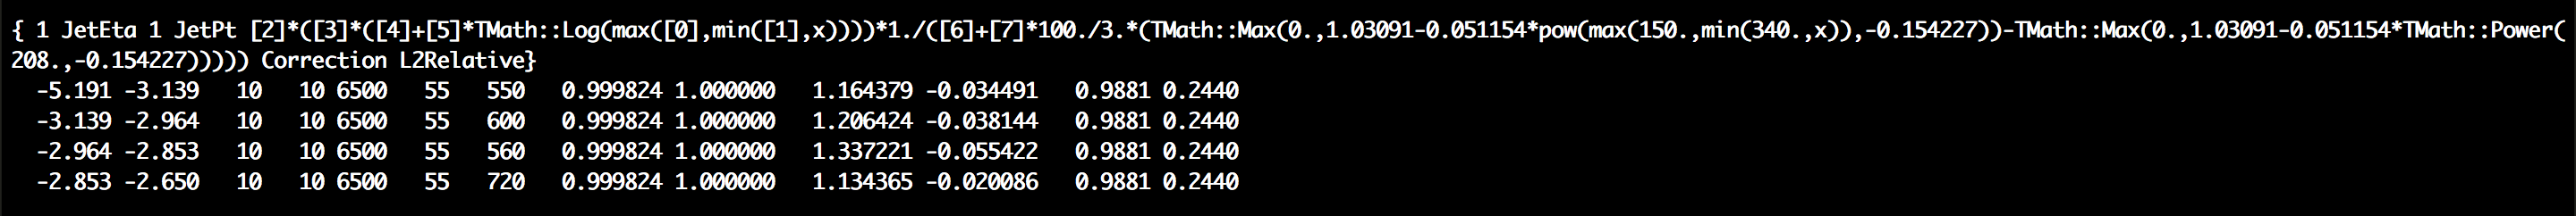
\includegraphics[width=\textwidth]{images/TextFileScreenshots/L2L3Residuals.png}    
                    \caption{L2L3Residuals}
                 \end{figure}

	\vspace{-.5cm}
	\begin{block}{How to read the JEC text files?}
                \begingroup \scriptsize
		\begin{itemize}
		\item The \textbf{top row} establishes the definitions for the parameters to follow, the correction factor and the correction level being applied.
		\item The \textbf{first two columns} are the $\eta$ bin boundaries
		\item The next column tells you how many columns will follow it (in this case 9)
		\item The next numbers define the bin boundaries in e.g. $\rho$, $p_{T}$, and/or jet area
                \item The last numbers are parameters for the correction
		\item Instructions on how to apply the Jet Energy Corrections from a text file in FWLite environment. \\ 
		\href{https://twiki.cern.ch/twiki/bin/view/CMSPublic/WorkBookJetEnergyCorrections}{https://twiki.cern.ch/twiki/bin/view/CMSPublic/WorkBookJetEnergyCorrections}
		\end{itemize}
                \endgroup
	\end{block}
}

\frame{
\frametitle{What form do the corrections come in?}
\framesubtitle{JEC Uncertainty Text Files}
                \begin{figure}
                  \centering
		     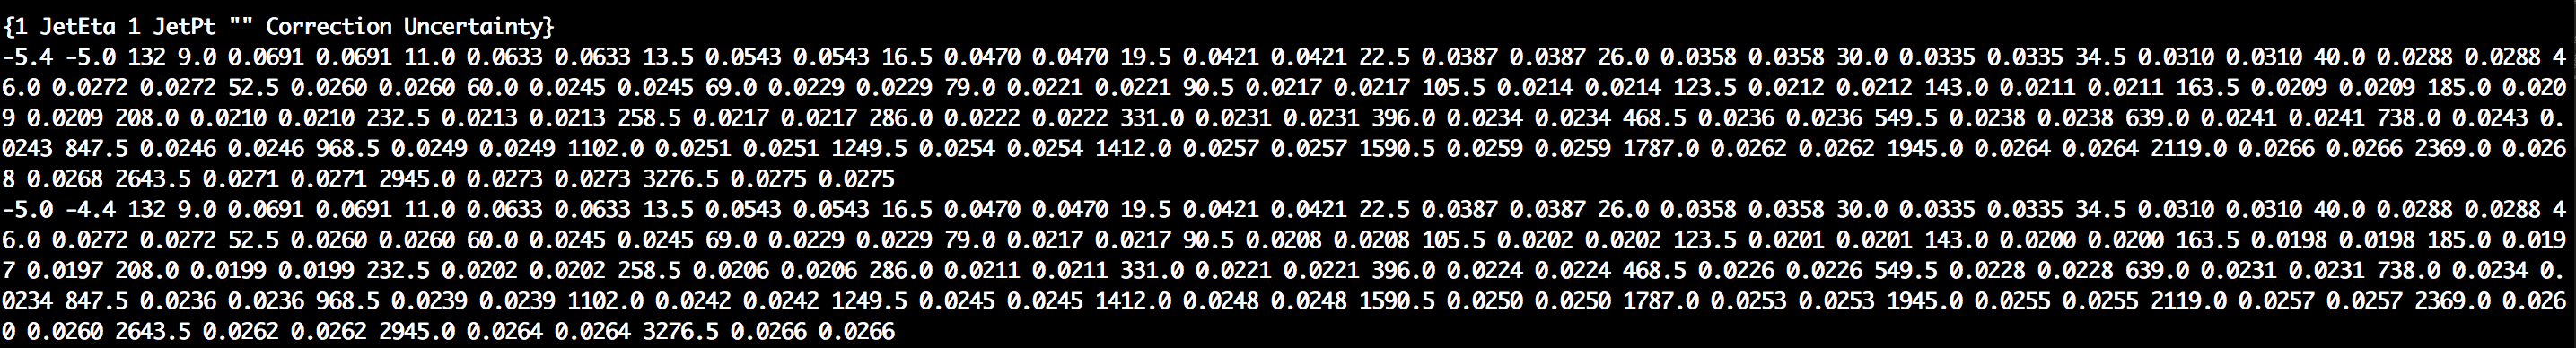
\includegraphics[width=\textwidth]{images/TextFileScreenshots/Uncertainty.png}    
                    \caption{Total Uncertainty}
                 \end{figure}
	\vspace{-.4cm}
                \begin{figure}
                  \centering
	             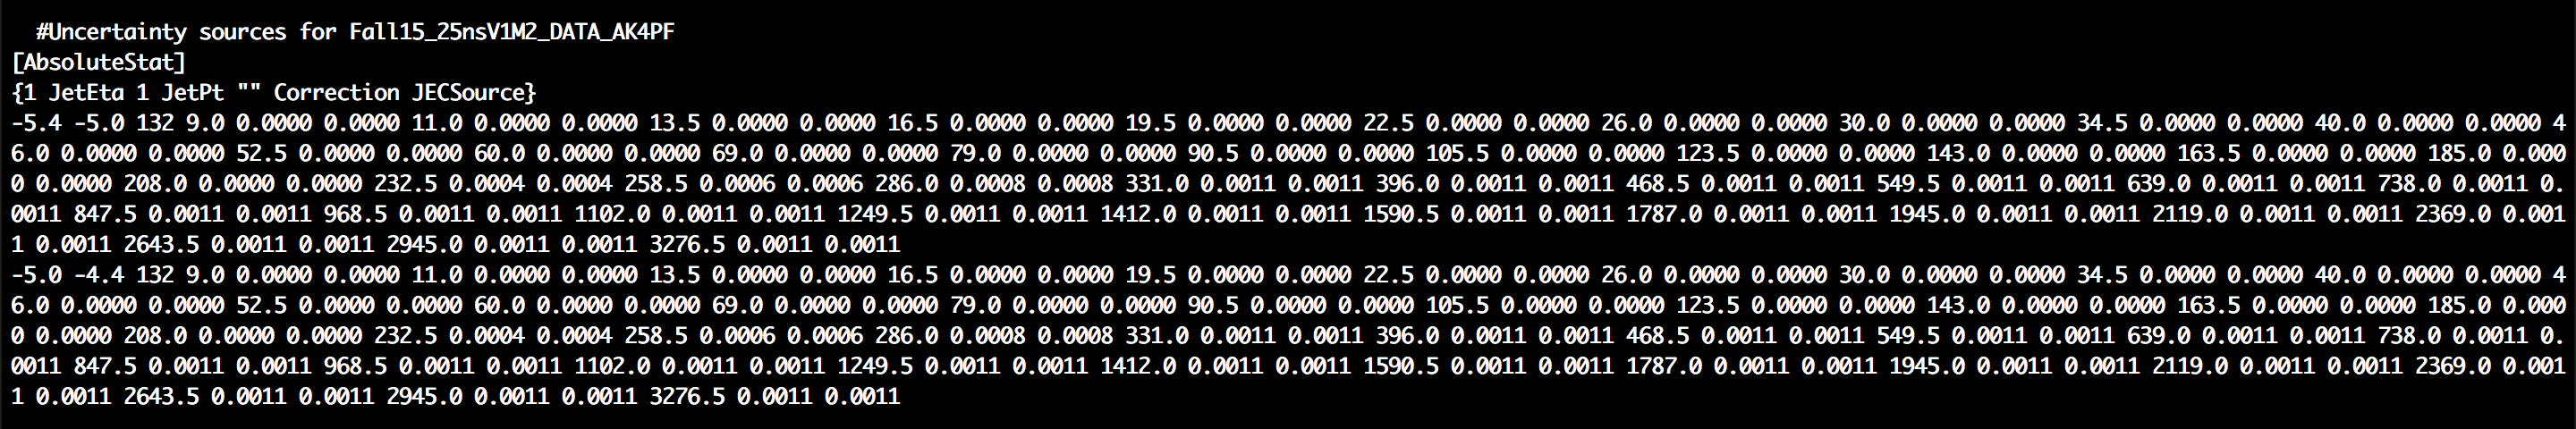
\includegraphics[width=\textwidth]{images/TextFileScreenshots/UncertaintySources.png}    
                    \caption{Uncertainty by Source}
                 \end{figure}

	\vspace{-.5cm}
	\begin{block}{How to read the JEC Uncertainty text files?}
                \begingroup \scriptsize
		\begin{itemize}
                \item First two columns are $\eta$ range, third column is how many columns will follow it
                \item Following this, you have lower $p_T$ bin boundary, uncertainty, upper $p_T$ bin boundary repeated
                \item In file with uncertainties split by source, the name of the source begins each section [LikeThis]
		\end{itemize}
                \endgroup
	\end{block}
}

\frame{
\frametitle{What form do the corrections come in?}
\framesubtitle{JER Text Files}
                \begin{figure}
                  \centering
		     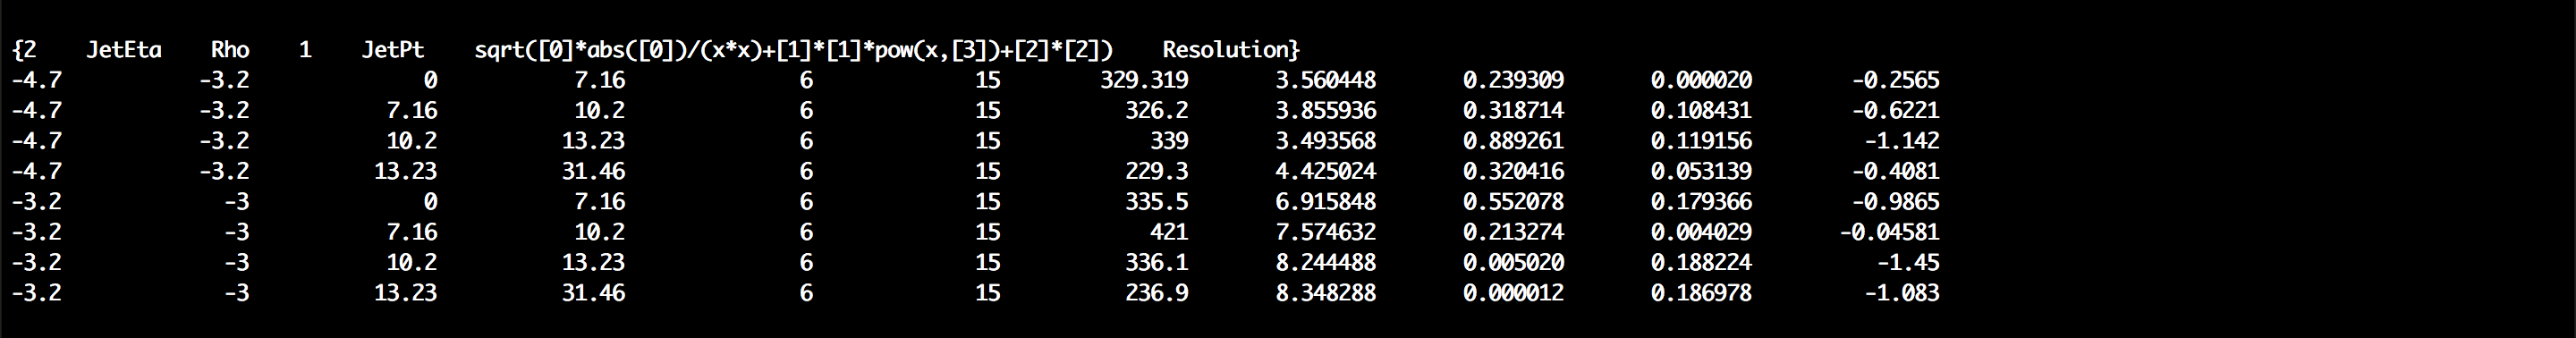
\includegraphics[width=\textwidth]{images/TextFileScreenshots/JetResolutionResolution.png}    
                    \caption{Jet Resolution}
                 \end{figure}
	\vspace{-.4cm}
                \begin{figure}
                  \centering
	             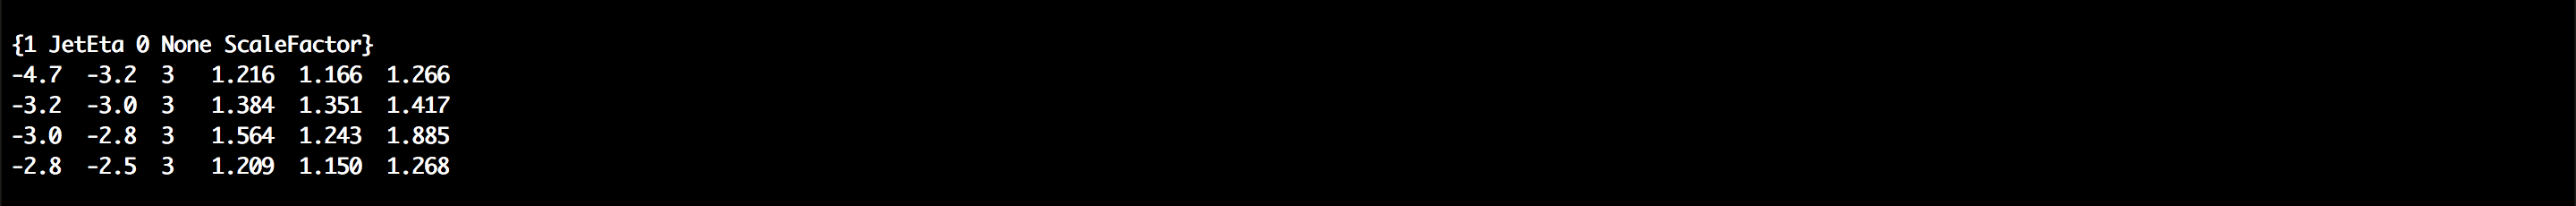
\includegraphics[width=\textwidth]{images/TextFileScreenshots/JetResolutionScaleFactors.png}    
                    \caption{Jet Resolution Scale Facors}
                 \end{figure}

	\vspace{-.5cm}
	\begin{block}{How to read the JER text files?}
                \begingroup \scriptsize
		\begin{itemize}
                \item JER (top): $\eta$ bin boundaries, rho bin boundaries, number of columns to follow, $p_T$ bin boundaries, parameters
                \item JER scale factors (bottom): $\eta$ bin boundaries, number of columns to follow, scale factor, scale factor varied down, scale factor varied up
		\end{itemize}
                \endgroup
	\end{block}
}

%-----------------------------------------------------------------------------------------------------------
\subsection{Textfile Application}
\frame{
\frametitle{What form do the corrections come in?}
\framesubtitle{Global Tag}
\begin{block}{Global Tag}
\begin{itemize}
\item Conditions data are defined in the Offline Conditions Database (ORCOF), which is read in CMSSW applications via Frontier caching servers.
\item The set of dataset tags which together define the offline conditions data are collected together in a \textbf{Global Tag (GT)}, which is itself stored in the database.
\item How to connect to a GT:
\end{itemize} 
\end{block}

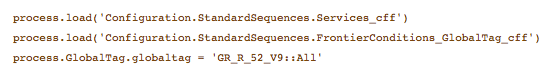
\includegraphics[width=10cm]{images/globaltag.png}

\begin{alertblock}{Note:}
\begin{itemize}
\item There can be many GT's for a given CMSSW release
\item It is important, therefore, that you know which conditions are in the GT you are using
\end{itemize}
\end{alertblock}

}
%-----------------------------------------------------------------------------------------------------------
\frame{
\frametitle{What form do the corrections come in?}
\framesubtitle{How to connect to a local sql file.}
\begin{columns}
\begin{column}{3.5cm}
\begin{block}{}
The recommended way of accessing JEC is with a global tag. The SQLlite file option is mainly used in the initial testing phase in preparation of a global tag.
\end{block}
\end{column}
\begin{column}{8.5cm}
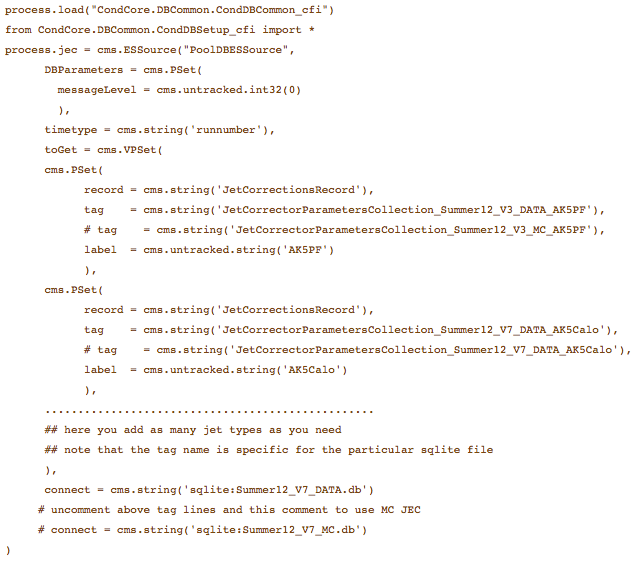
\includegraphics[width=8.5cm]{images/sqlfile.png}
\end{column}
\end{columns}

}
%-----------------------------------------------------------------------------------------------------------
\frame{
\frametitle{What form do the corrections come in?}
\framesubtitle{How to connect to a local sql file.}

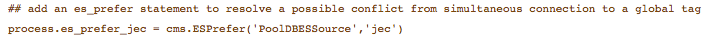
\includegraphics[width=11cm]{images/sql2.png}

\begin{block}{}
\begin{itemize}
\item When using a local SQL file, \textbf{es$\_$prefer} should be added to the process chain in the cfg file.
\item In this case, an \textbf{es$\_$prefer} indicates that whatever is defined in \textbf{es$\_$source} takes precedence over any other source for the condition object (in particular, the global tag).
\end{itemize}
\end{block}

}





